% The "%" character denotes a comment
% This file was written by Nathan Moore, Winona State University
% as a template for how lab reports might be written in LaTeX.
% style choices originally come from the American Journal of Physics's
% sample submission file, http://ajp.dickinson.edu/Contributors/manFormat.html
%
%
\documentclass[prb,preprint]{revtex4-1}
\usepackage{amsmath}  % needed for \tfrac, \bmatrix, etc.
\usepackage{amsfonts} % needed for bold Greek, Fraktur, and blackboard bold
\usepackage{graphicx} % needed for figures

%these are some macros (shortcuts)
\newcommand{\bea}{\begin{eqnarray}}
\newcommand{\eea}{\end{eqnarray}}
\newcommand{\be}{\begin{equation}}
\newcommand{\ee}{\end{equation}}

\usepackage{rotating}


\begin{document}

\title{Throughput Testing on the HP Elitebook G2}
\author{Adam Stammer}
\date{\today}

\maketitle
	
\section{Brief Analysis}

The first graph below shows the result of a rather extreme throughput test. You can see that this test went all the way up to 500 threads and did so rather quickly at 20 threads added every 5 seconds. This test was not really meant to show detail of throughput but an overview such that I might narrow down a decent maximum thread count to use in my detailed tests. I decided that throughput was relatively linear up until 200 threads and nearly capped out at 300 threads. I wanted to capture detail in both of these regions so I deemed 300 threads to be an acceptable max thread count.
\linebreak
From there I ran four tests, altering 2 binary variables, whether or not the computer was plugged in, and whether the cpu frequency was dynamic or fixed at it's maximum, 2.71GHz in the case of this HP Elitebook G2. Each test was run close to 300 threads, until there were 3 measurements of 100\% cpu utilization. I chose a continuous line graph for showing CPU utilization because it adds a depth of time which is otherwise not communicated but a rather important feature of this measurement.


A brief analysis of these graphs leads me to three main takeaways:
\begin{enumerate}
	\item Plugging the computer in tends to raise the ceiling of throughput
	\item Dynamic CPU frequency makes CPU utilization rather erratic likely due to a difficulty in measurement
	\item Transaction/Second count tends to fall off shortly before 100\% CPU utilization is reached
\end{enumerate}

\begin{sidewaysfigure}
	\centering
	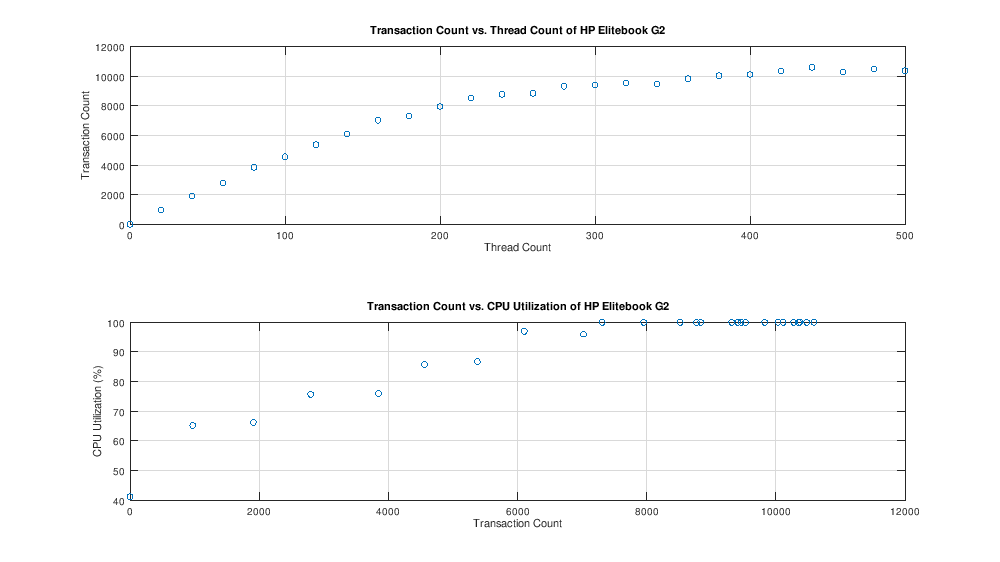
\includegraphics[width=10in]{bigGraphInitial.png}
	\caption{Extreme run used to decide range}
	\label{fig1}
\end{sidewaysfigure}

\begin{sidewaysfigure}
		\centering
		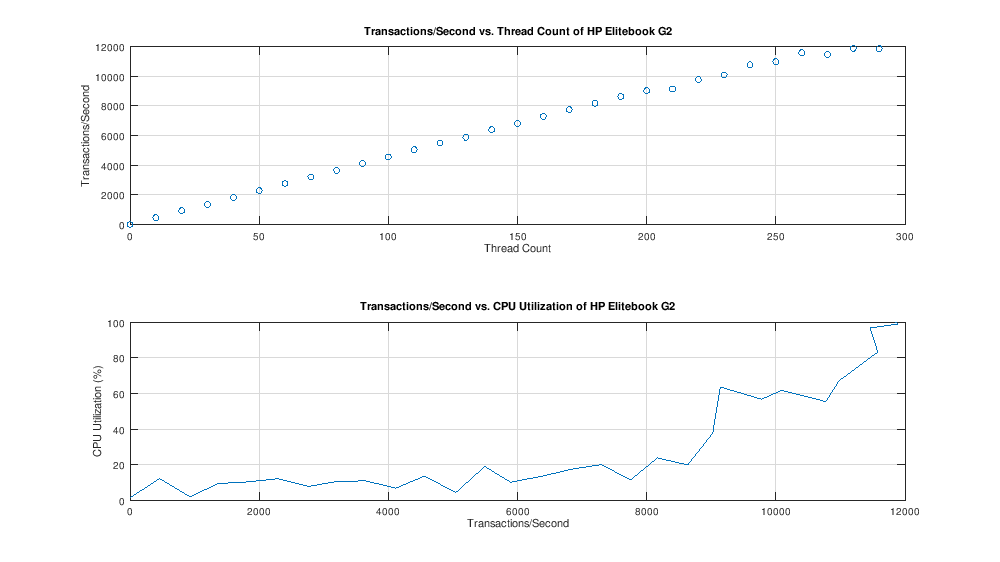
\includegraphics[width=10in]{FixedMaxPluggedIn.png}
		\caption{Fixed Maximum Frequency, Plugged In}
		\label{fig1}
\end{sidewaysfigure}

\begin{sidewaysfigure}
\centering
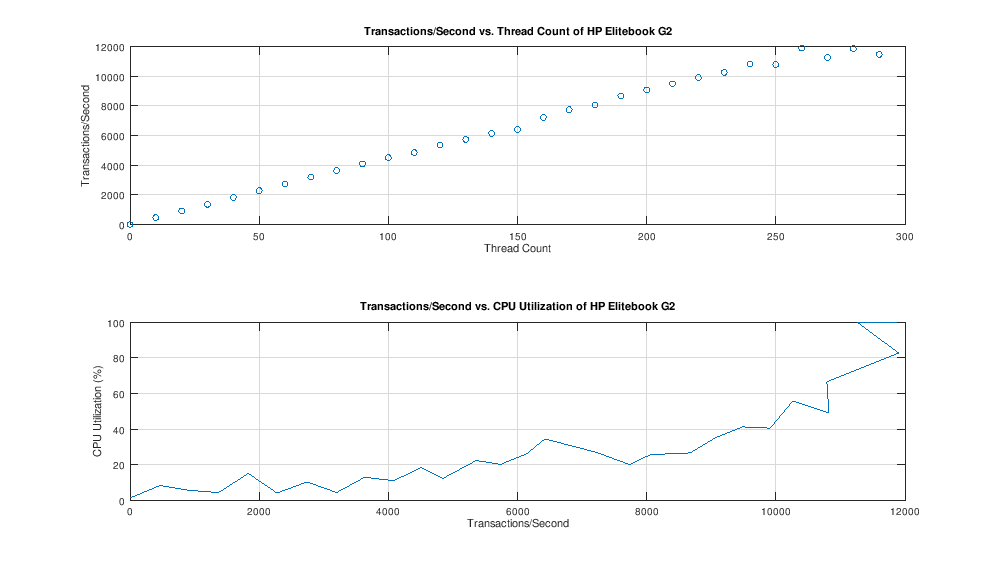
\includegraphics[width=10in]{FixedMaxBattery.png}
\caption{Fixed Maximum Frequency, Battery}
\label{fig1}
\end{sidewaysfigure}

\begin{sidewaysfigure}
\centering
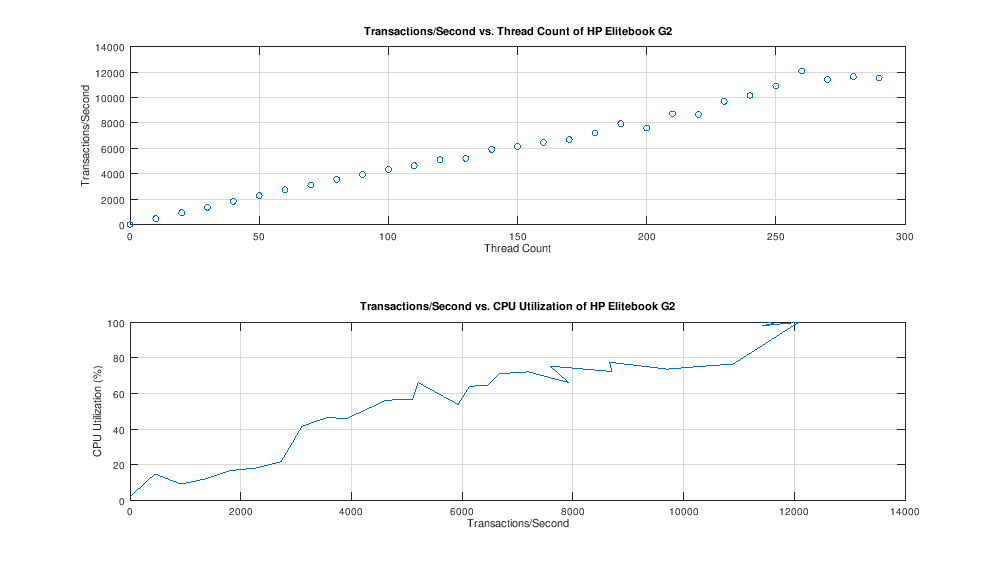
\includegraphics[width=10in]{DynamicPluggedIn.png}
\caption{Dynamic Frequency, Plugged In}
\label{fig1}
\end{sidewaysfigure}

\begin{sidewaysfigure}
\centering
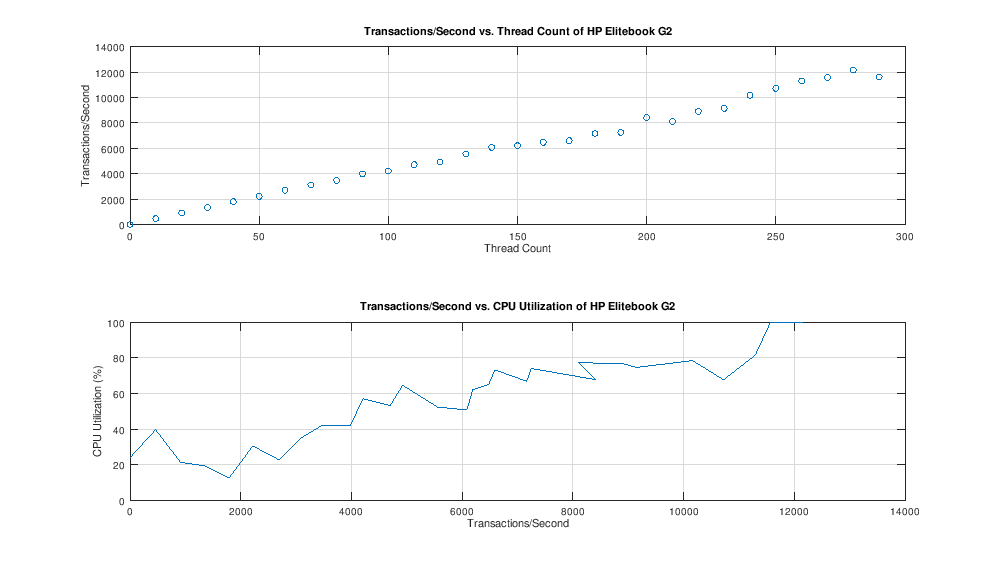
\includegraphics[width=10in]{DynamicBattery.png}
\caption{Dynamic Frequency, Battery}
\label{fig1}
\end{sidewaysfigure}


\end{document}
